\documentclass{article}

\usepackage{graphicx}
\usepackage{amsmath}
\usepackage[margin=3cm]{geometry}



\begin{document}
\section{ Some simple notes}

\subsection{ Normality check}
\begin{figure}[h]
%    \centering
    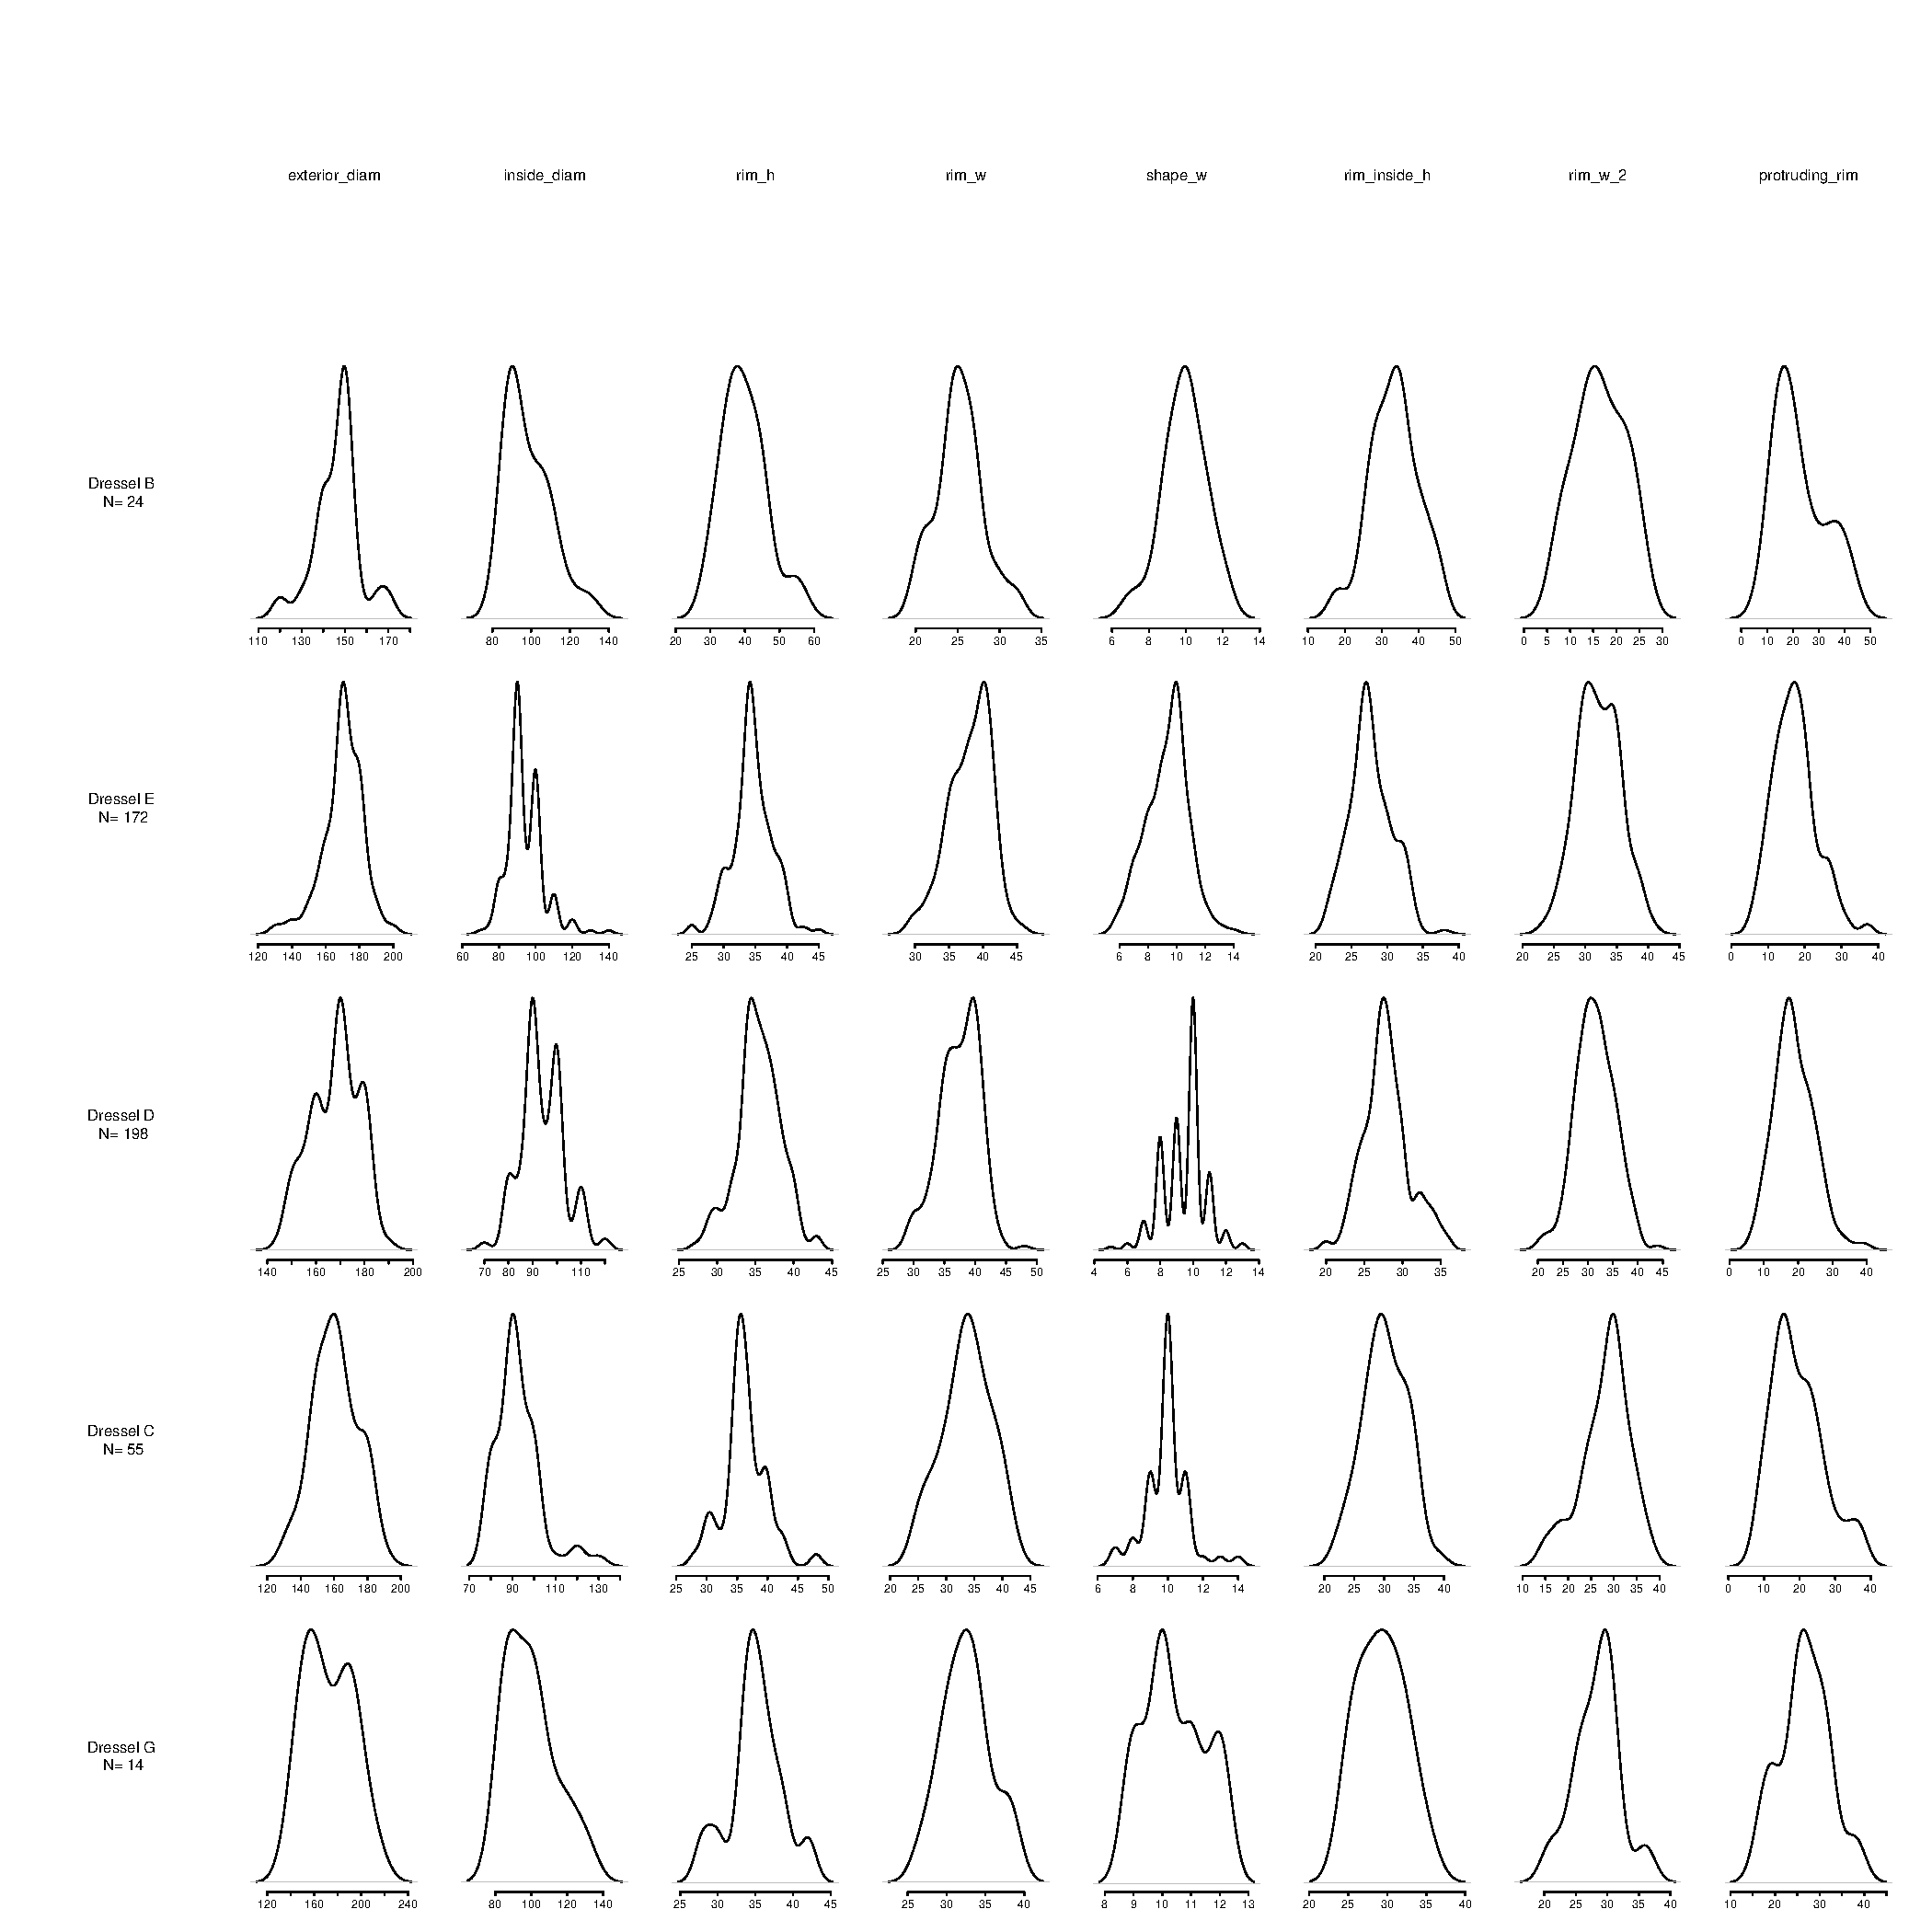
\includegraphics[width=\textwidth]{distrib_allmeasurment_dresseltype.pdf}
%    \caption{Distribution of measurement for all types of dressels}
\end{figure}

\subsubsection{Univariate test for all measurment and for all types}
% latex table generated in R 3.3.3 by xtable 1.8-2 package
% Sat Apr 28 18:49:52 2018
\begin{table}[ht]
\centering
\begin{tabular}{llllll}
  \hline
Test & Variable & Statistic & p value & Normality & type \\ 
  \hline
Shapiro-Wilk & exterior\_diam  &    0.9030 &    0.0250 &    NO     & Dressel B \\ 
  Shapiro-Wilk &  inside\_diam   &    0.8858 &    0.0109 &    NO     & Dressel B \\ 
  Shapiro-Wilk &     rim\_h      &    0.9488 &    0.2551 &    YES    & Dressel B \\ 
  Shapiro-Wilk &     rim\_w      &    0.9666 &    0.5837 &    YES    & Dressel B \\ 
  Shapiro-Wilk &    shape\_w     &    0.9298 &    0.0965 &    YES    & Dressel B \\ 
  Shapiro-Wilk &  rim\_inside\_h  &    0.9784 &    0.8656 &    YES    & Dressel B \\ 
  Shapiro-Wilk &    rim\_w\_2     &    0.9609 &    0.4562 &    YES    & Dressel B \\ 
  Shapiro-Wilk & protruding\_rim &    0.8936 &    0.0158 &    NO     & Dressel B \\ 
  Shapiro-Wilk & exterior\_diam  &    0.9390 &  $<$0.001   &    NO     & Dressel E \\ 
  Shapiro-Wilk &  inside\_diam   &    0.8956 &  $<$0.001   &    NO     & Dressel E \\ 
  Shapiro-Wilk &     rim\_h      &    0.9759 &  0.0043   &    NO     & Dressel E \\ 
  Shapiro-Wilk &     rim\_w      &    0.9688 &   7e-04   &    NO     & Dressel E \\ 
  Shapiro-Wilk &    shape\_w     &    0.9476 &  $<$0.001   &    NO     & Dressel E \\ 
  Shapiro-Wilk &  rim\_inside\_h  &    0.9678 &   5e-04   &    NO     & Dressel E \\ 
  Shapiro-Wilk &    rim\_w\_2     &    0.9879 &  0.1453   &    YES    & Dressel E \\ 
  Shapiro-Wilk & protruding\_rim &    0.9721 &  0.0016   &    NO     & Dressel E \\ 
  Shapiro-Wilk & exterior\_diam  &    0.9450 &  $<$0.001   &    NO     & Dressel D \\ 
  Shapiro-Wilk &  inside\_diam   &    0.9467 &  $<$0.001   &    NO     & Dressel D \\ 
  Shapiro-Wilk &     rim\_h      &    0.9782 &  0.0035   &    NO     & Dressel D \\ 
  Shapiro-Wilk &     rim\_w      &    0.9711 &   4e-04   &    NO     & Dressel D \\ 
  Shapiro-Wilk &    shape\_w     &    0.9314 &  $<$0.001   &    NO     & Dressel D \\ 
  Shapiro-Wilk &  rim\_inside\_h  &    0.9706 &   4e-04   &    NO     & Dressel D \\ 
  Shapiro-Wilk &    rim\_w\_2     &    0.9907 &  0.2331   &    YES    & Dressel D \\ 
  Shapiro-Wilk & protruding\_rim &    0.9782 &  0.0036   &    NO     & Dressel D \\ 
  Shapiro-Wilk & exterior\_diam  &    0.9602 &  0.0661   &    YES    & Dressel C \\ 
  Shapiro-Wilk &  inside\_diam   &    0.8486 &  $<$0.001   &    NO     & Dressel C \\ 
  Shapiro-Wilk &     rim\_h      &    0.9502 &  0.0236   &    NO     & Dressel C \\ 
  Shapiro-Wilk &     rim\_w      &    0.9736 &  0.2655   &    YES    & Dressel C \\ 
  Shapiro-Wilk &    shape\_w     &    0.8799 &   1e-04   &    NO     & Dressel C \\ 
  Shapiro-Wilk &  rim\_inside\_h  &    0.9835 &  0.6491   &    YES    & Dressel C \\ 
  Shapiro-Wilk &    rim\_w\_2     &    0.9522 &  0.0286   &    NO     & Dressel C \\ 
  Shapiro-Wilk & protruding\_rim &    0.9460 &  0.0154   &    NO     & Dressel C \\ 
  Shapiro-Wilk & exterior\_diam  &    0.9308 &    0.3126 &    YES    & Dressel G \\ 
  Shapiro-Wilk &  inside\_diam   &    0.8943 &    0.0931 &    YES    & Dressel G \\ 
  Shapiro-Wilk &     rim\_h      &    0.9711 &    0.8913 &    YES    & Dressel G \\ 
  Shapiro-Wilk &     rim\_w      &    0.9661 &    0.8200 &    YES    & Dressel G \\ 
  Shapiro-Wilk &    shape\_w     &    0.8802 &    0.0585 &    YES    & Dressel G \\ 
  Shapiro-Wilk &  rim\_inside\_h  &    0.9584 &    0.6960 &    YES    & Dressel G \\ 
  Shapiro-Wilk &    rim\_w\_2     &    0.9556 &    0.6500 &    YES    & Dressel G \\ 
  Shapiro-Wilk & protruding\_rim &    0.9719 &    0.9008 &    YES    & Dressel G \\ 
   \hline
\end{tabular}
\end{table}


We tested the normality of the distribution for all the the differents differents dressel type. Lot of the measurments \emph{are not} distributed normally \emph{but}, it may du to various reason: the we took all the workshop and all the chronologies togehr. This often gives some multimodal distributions which rejects the normality test though it may be the composition of two normal distributions.  

Moreover, the rim\_w\_2  measuremnt is normal for ALL types, which may detect a really good standardisation for this part of the amphorae.  

\subsubsection{Multivariate test for all measurment and for all types}
If no one of the dressel type seems to pass the multivariate normality test it's remarkable to see that in some case, they do. It's remarkable as, as we already said, the test are grouping together amphoraes from all the workshop and from different chronologies.
% latex table generated in R 3.3.3 by xtable 1.8-2 package
% Sat Apr 28 18:49:53 2018
\begin{table}[ht]
\centering
\begin{tabular}{lllll}
  \hline
Test & Statistic & p value & Result & type \\ 
  \hline
Mardia Skewness & 151.00326890286 & 0.029167986889231 & NO & Dressel B \\ 
  Mardia Kurtosis & 0.733728310309191 & 0.463114340679657 & YES & Dressel B \\ 
  MVN &  &  & NO & Dressel B \\ 
  Mardia Skewness & 276.872528485622 & 2.02752220168503e-14 & NO & Dressel E \\ 
  Mardia Kurtosis & 4.72467285683036 & 2.30486093144577e-06 & NO & Dressel E \\ 
  MVN &  &  & NO & Dressel E \\ 
  Mardia Skewness & 190.808852630645 & 4.17346199684803e-05 & NO & Dressel D \\ 
  Mardia Kurtosis & 2.76709956273982 & 0.00565574794696677 & NO & Dressel D \\ 
  MVN &  &  & NO & Dressel D \\ 
  Mardia Skewness & 157.161262154261 & 0.0128707519935051 & NO & Dressel C \\ 
  Mardia Kurtosis & 1.23577005038261 & 0.216544050552106 & YES & Dressel C \\ 
  MVN &  &  & NO & Dressel C \\ 
  Mardia Skewness & 138.125922212595 & 0.123361105954831 & YES & Dressel G \\ 
  Mardia Kurtosis & -0.939044316308594 & 0.34770799172399 & YES & Dressel G \\ 
  MVN &  &  & YES & Dressel G \\ 
   \hline
\end{tabular}
\end{table}


Even if some test are negatives, their is numerous hint telling us tha indeed the measurments of the amphora are randomly distributed. We will them base the model on this assumptions.

\section{Continuous Distance Biased Copy}
Remarques: in this section all the distances dsicuted are \emph{relative} distance. They are distances normalized such as all distance are between 0 and 1.

\subsection{Idea}
  We want to test : what kind of cultural transmission can reproduce the data. More precisely: how the distance impact this tranmission.
The idea is to propose a single parameter that allows to explore this  and to avoid three adhoc model.

So let's introduce a new parameter $\alpha \in [-1,1]$ that will do this job and that will control impact of the distance on the cultural transmission mechanism. 

\subsection{Previously}
We first proposed three distinct mechanisms:
\begin{enumerate}
    \item Horizontal Transmission: the workers from all workshop can copy eachother, regadless the distance they are from the worker in other workshop
    \item Vertical Transmission: the workers cannot move frome on workshop to another
    \item Oblique transmission: the workers can move and tend to move more frequently to the workshop closer to where they are working
\end{enumerate}
Those three scenarios are transformed in three probabilities that two workshop $i$ \& $j$ to copy each other:
\begin{enumerate}
    \item $p_{i,j}=\mu$ (HT : all workshop have the same probability to copy eachother))
    \item $p_{i,j}=0$ (VT: workshop are not copying eachother)
    \item $p_{i,j}=\mu \time D(i,j)$ (HT:the probability of 2 worrkshops to copy eachother depends on the distance between the 2 WS)
\end{enumerate}

\subsection{New and unique parameters $\alpha$}
The idea is now to go accross all possible value of this paramter using ABC.


To introduce the new parameter we created a new function $\beta_d(d_{i,j},\alpha)$, were $d_{i,j}$ is the distance between two workshop $i$ and $j$ and $\alpha$ our new paramater, which can be interpretad at the strenght of the distance.
Obviously this function should be able to reproduce the three previous scenarios. We can rewrite the previous probabilities including $\alpha$ and we should have:
\begin{enumerate}
    \item $p_{i,j,\alpha_a}=\mu$ (HT : all workshop have the same probability to copy eachother))
    \item $p_{i,j,\alpha_b}=0$ (VT: workshop are not copying eachother)
    \item $p_{i,j,\alpha_c}=\mu \time (1-D(i,j))$ (HT:the probability of 2 worrkshops to copy eachother depends on the distance between the 2 WS)
\end{enumerate}
We choose: $\alpha_a=0,\alpha_c=1,\alpha_b=-1$ and thus define $\alpha \in [-1,1]$. One we to see that is to say that one alpha is at 1, the impact of distance is maximum \emph{ie} if any distance more that 0 is infinitely long to travel.   This is the Vertical Transmision case. When $\alpha$ is 0 the strenght of the bias is null, then the proability is directly proportional to the distance. If $\alpha=-1$ then the strength of bias is negative \emph{ie} the distance have no impact on the probability to copy someonells. This is the Horizontal transmission case. 

The idea is to find a function taht allows to pass from one scenario to another with intermediate situation (the bias is strong but no so much: you can still copy the people not so far from you\ldots)
To implemante that we propose the function $\beta_d(d_{i,j},\alpha)$ that transform the distance $d_{i,j}$ given the strenght of the bias $\alpha$
\begin{equation}
    \beta_d(d_{i,j},\alpha):
    1-(1-{d_{i,j}})^{100^\alpha}
\end{equation}


The figure~\ref{fig:betaforxalphas} shows how the distance are transformated by our function given some differents $\alpha$
\begin{figure}[h]
    \centering
    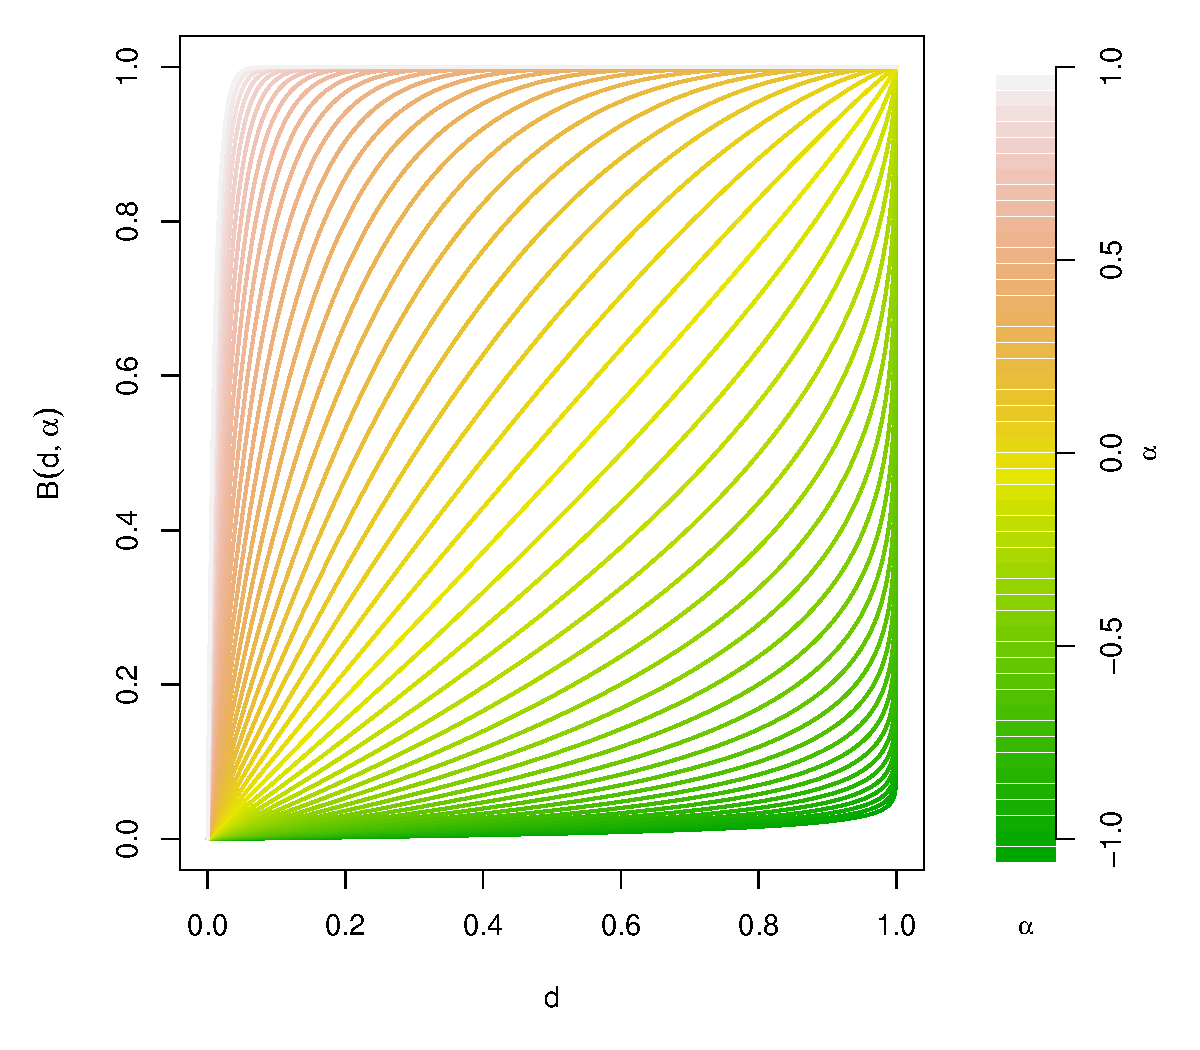
\includegraphics[width=.4\textwidth]{beta_alpha.pdf}
    \caption{Representation of $\beta_d$ for 50 $\alpha \in [-1,1]$ }
    \label{fig:betaforxalphas}
\end{figure}

We can now integrate $\alpha$ to the probability that one workshop $i$ copy another workshop $j$ as :
\begin{subequations}
    \begin{align}
        p_{i,j} = \mu \time \left( 1 - \beta_d(d_{i,j},\alpha)\right)\\
        p_{i,j} = \mu \time \left( 1 - 1 - (1 - {d_{i,j}})^{100^\alpha}\right)\\
        p_{i,j} = - \mu \time \left( {d_{i,j}}^{100^\alpha}\right)
    \end{align}

    \label{equ:probacopyalpha}
\end{subequations}

Know that we know for each $\alpha$ how to compute the probabilities, we show in the figure~\ref{fig:proba} shows how those probabilites are distributed given the distance and all the possible alphas.

\begin{figure}[h]
    \centering
    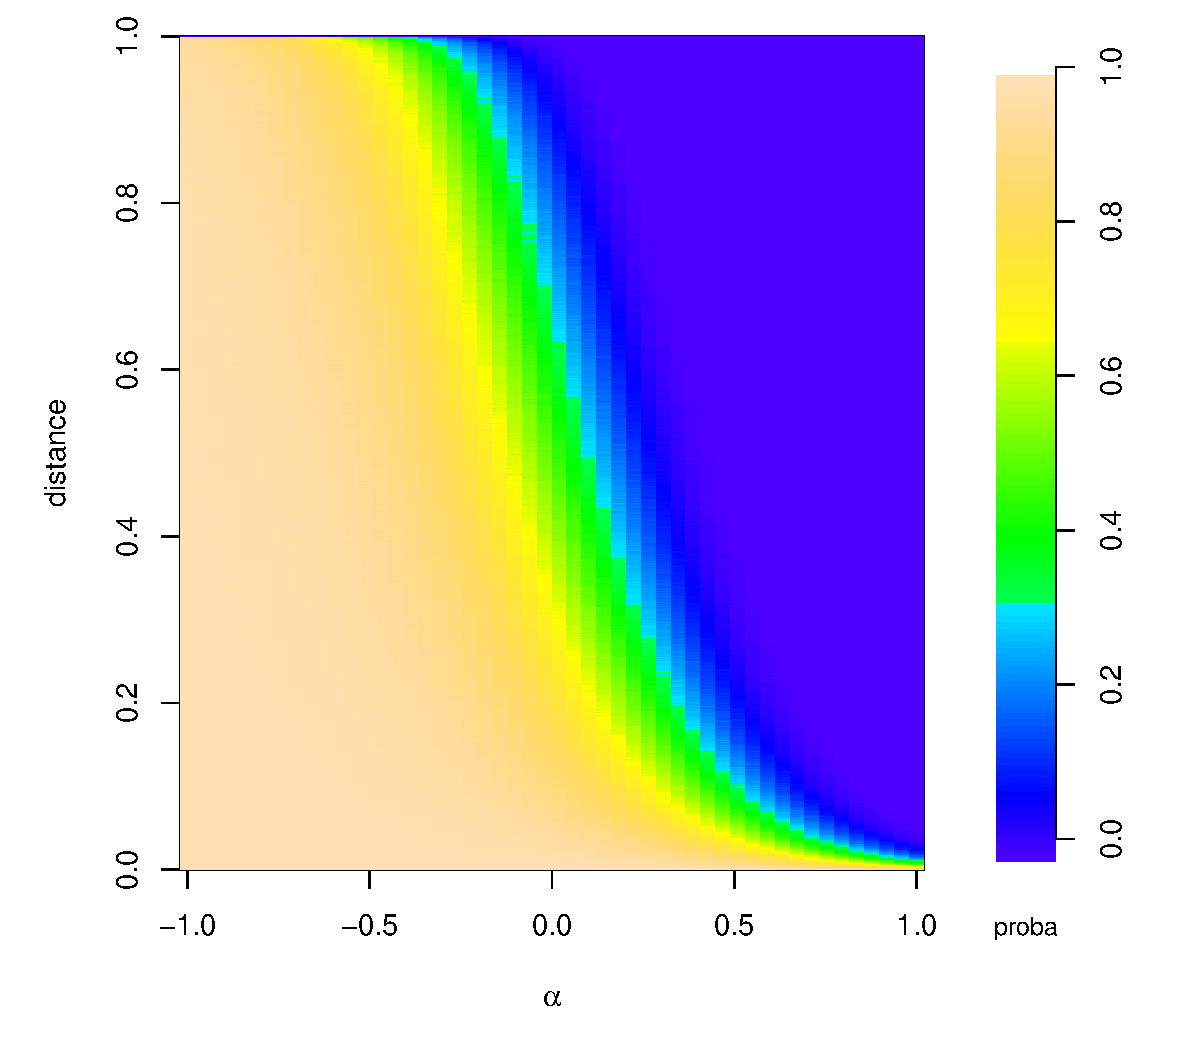
\includegraphics[width=.4\textwidth]{proba_map.pdf}
    \caption{Distributions of probabilites for all alpha and all distance}
    \label{fig:proba}
\end{figure}

We can see how the new function reproduces our 2 previous seniarios. All the left, yellow partm on the figure~\ref{fig:proba}, where all the probability are $1$ regardless to the distance correspond to our previous \emph{Horizontal Transfer(HT)}, all the right, blue part, where the probability is $0$ regaldless of the distance correspond to our previous \emph{Vertical Transfer(HT)}. On the middle ligne where $\alpha=0$, on can see that the probability is directly proportional to the distance, which represent or previous oblique transfer scenario. 

On can check this be looking at the next graph that plot the distribution of probabilites for the three cases described before.
\begin{figure}[h]
    \centering
    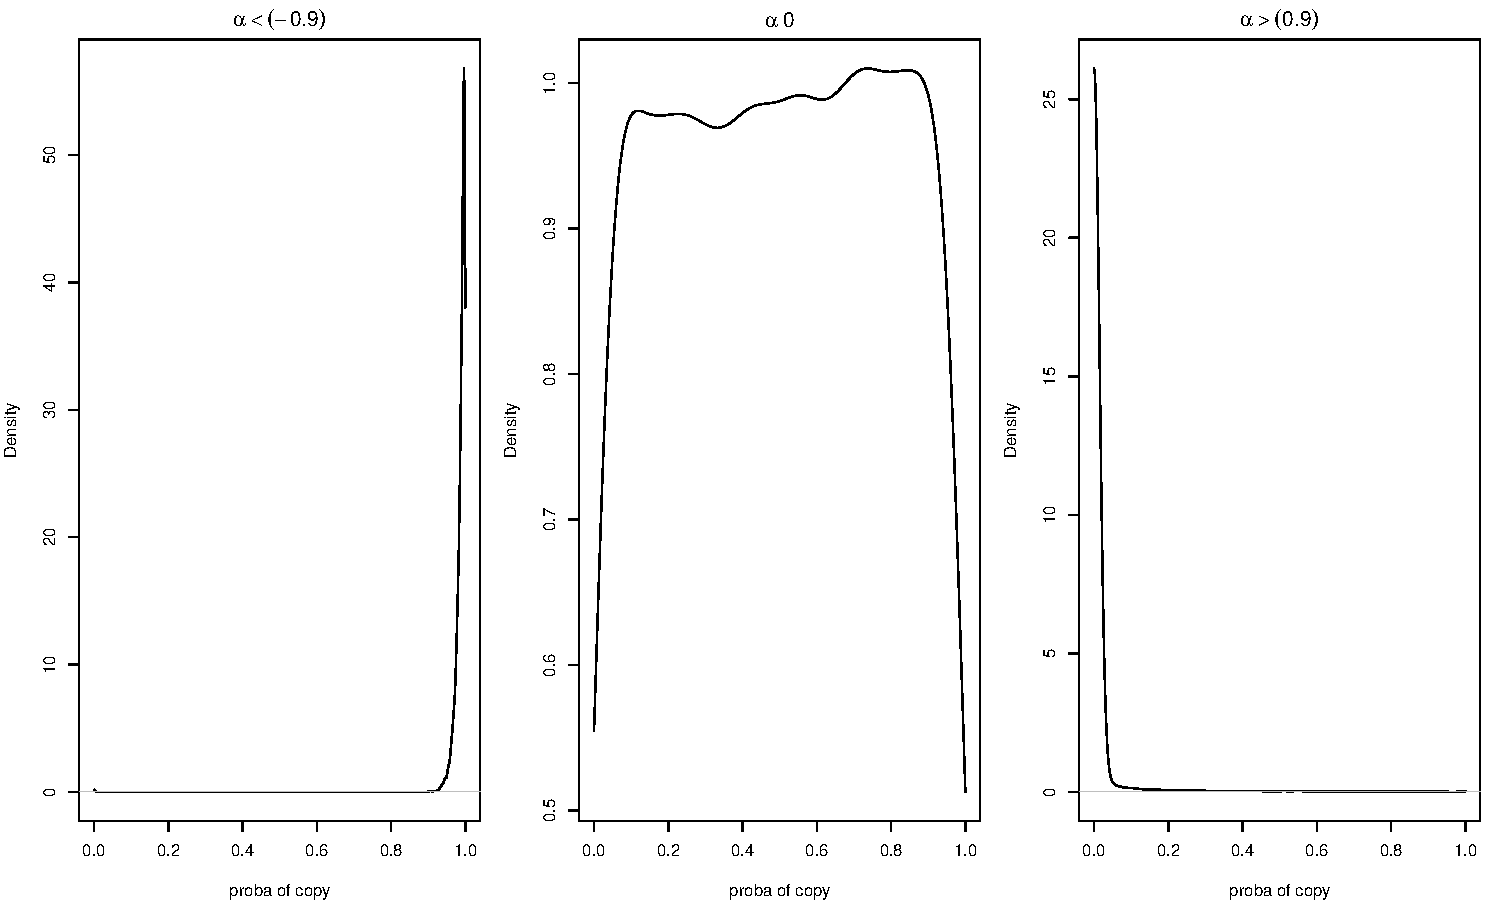
\includegraphics[width=.6\textwidth]{distribution_proba.pdf}
    \caption{reproduction of our three scenarios}
    \label{fig:thrreprob}
\end{figure}

\end{document}



